\chapter{Krachten op het schip}
\vspace{-120px}
\question{1}{Hoe zorg je ervoor dat je boot sneller oploeft?}
\answerTextFour{Door meer mensen aan de lijkant te zetten (lage kant)}{Door meer mensen aan de loefkant te zetten (hoge kant)}{Door je zwaard op te doen}{Door je grootzeil te vieren}


\question{2}{Wat is er fout aan het zeil in het figuur hiernaast?}
	\vspace{-20px}
\begin{figure}[H]		
	\begin{minipage}[]{0.70\textwidth}
		\begin{enumerate}[topsep=0pt, label=\Alph*.]
			\item Het zeil staat te strak
			\item Het zeil staat te los
			\item Het zeil is slecht gehesen
			\item Het zeil is kapot
		\end{enumerate}
	\end{minipage}
	\begin{minipage}[]{0.29\textwidth}
		\begin{figure}[H]
			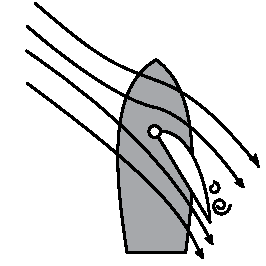
\includegraphics[width=0.80\textwidth,right]{Hoofdstukken/Krachten/pdf/zeil_strak.pdf}
		\end{figure}
	\end{minipage}
	\vspace{-20px}
\end{figure}



\question{3}{Je vaart halve wind en wil snel oploeven, wat doe je?}
\answerTextFour{Beide zeilen vieren}{Je fok vieren en grootzeil aantrekken}{Je grootzeil vieren en fok aantrekken }{Beide zeilen aantrekken}

\question{4}{Hoe controleer je of je grootzeil goed staat?}
\answerTextFour{Door je zeil te laten vieren}{Door deze te laten vieren tot hij tegenbolt en daarna een klein beetje aan te trekken}{Door een beetje af te vallen}{Door naar je zeillatjes te kijken}

\question{5}{Hoe kan je zien dat je zeil te los staat?}
\answerTextFour{Je gaat sneller varen}{Het voorlijk van je zeil gaat tegenbollen}{Je fok bolt tegen}{Het achterlijk van je zeil gaat klapperen}